\documentclass[11pt,a4paper]{report} 
% Alternativ für doppelseitigen Ausdruck (nur bei > 60 Seiten sinnvoll)
%\documentclass[11pt,a4paper,twoside,openright]{report}

% Deutsch
\usepackage[german]{babel} % deutsch und deutsche Rechtschreibung
\usepackage[utf8]{inputenc} % Unicode Text 
\usepackage[T1]{fontenc} % Umlaute und deutsches Trennen
\usepackage{textcomp} % Euro
\usepackage[hyphens]{url}
% statt immer Ab\-schluss\-ar\-beit zu schreiben
% einfach hier sammeln mit -. 
\hyphenation{Ab-schluss-ar-beit}
% Vorsicht bei Umlauten und Bindestrichen
\hyphenation{Ver-st\"ar-ker-aus-gang}
 % eigene Hyphenations, die für das Dokument gelten
\usepackage{amssymb} % Symbole
\usepackage{enumitem}
\usepackage{tabularx}


%% Fonts, ein kompletter Satz an Optionen
% Times New Roman, gewohnter Font mit ok tt und serifenlos
%\usepackage{mathptmx} 
%\usepackage[scaled=.95]{helvet}
%\usepackage{courier}
% Palatino, mal was anderes, auch mit ok tt und serifenlos
% empfohlen
\usepackage{mathpazo} % Palatino, mal was anderes
\usepackage[scaled=.95]{helvet}
\usepackage{courier}
% New Century Schoolbook sieht auch nett aus (macht auch tt und serifenlos)
%\usepackage{newcent}

% zusätzlich: Default serifenlos mit Helvetica 
% ich kann es nicht mehr sehen...
%\renewcommand{\familydefault}{\sfdefault}

\usepackage{microtype}

% Bilder und Listings
\usepackage{graphicx} % wir wollen Bilder einfügen
\usepackage{subfig} % Teilbilder
\usepackage{wrapfig} % vielleicht doch besser vermeiden
\usepackage{listings} % schöne Quellcode-Listings
% ein paar Einstellungen für akzeptable Listings
\lstset{basicstyle=\sffamily, columns=[l]flexible, mathescape=true, showstringspaces=false, numbers=left, numberstyle=\tiny}
\lstset{language=python} % und nur schöne Programmiersprachen ;-)
% und eine eigene Umgebung für Listings
\usepackage{float}
\newfloat{listing}{htbp}{scl}[chapter]
\floatname{listing}{Listing}

% Seitenlayout
%\usepackage[paper=a4paper,width=14cm,left=35mm,height=22cm]{geometry}
\usepackage[paper=a4paper,width=14cm,height=22cm]{geometry}
\usepackage{setspace}
\linespread{1.15}
\setlength{\parskip}{0.5em}
\setlength{\parindent}{0em} % im Deutschen Einrückung nicht üblich, leider

% Seitenmarkierungen 
\newcommand{\phv}{\fontfamily{phv}\fontseries{m}\fontsize{9}{11}\selectfont}
\usepackage{fancyhdr} % Schickere Header und Footer

\pagestyle{fancy}
\renewcommand{\chaptermark}[1]{\markboth{#1}{}}
\renewcommand{\sectionmark}[1]{\markright{#1}}
\fancyhead[LO]{\phv \nouppercase{\leftmark}}
\fancyhead[RE]{\phv \nouppercase{\rightmark}}
\fancyhead[RO,LE]{\phv \thepage}
\fancyfoot[C]{\ } % Seitenzahl unten nur Kapitel


% Theorem-Umgebungen
\newtheorem{definition}{Definition}[chapter]
\newtheorem{satz}{Satz}[chapter]
\newtheorem{lemma}[satz]{Lemma} % gleicher Zähler wie Satz
\newtheorem{theorem}{Theorem}[chapter]
\newenvironment{beweis}[1][Beweis]{\begin{trivlist}
\item[\hskip \labelsep {\textit{#1 }}]}{\end{trivlist}}
\newcommand{\qed}{\hfill \ensuremath{\square}}

% Inhaltsverzeichnis
\setcounter{tocdepth}{1}
\setcounter{secnumdepth}{2}

% Quellen teilen
\usepackage{bibtopic} 

% Hochschule Logo, noch nicht perfekt
\usepackage{hsrmlogo}

% Spezialpakete
\usepackage{epigraph}
\setlength{\epigraphrule}{0pt} % kein Trennstrich

% damit wir nicht so viel tippen müssen, nur für Demo 
\usepackage{blindtext} 

% Zum Zeigen von Fehlern
\usepackage{soul}
\newcommand*\falsch{\st}

% Links im PDF
\usepackage{hyperref}
\hypersetup{
    colorlinks=true,
    citecolor=black,
    filecolor=black,
    linkcolor=black,
    urlcolor=black
}

% Kommentare
\usepackage{comment} % alle Pakete und Einstellungen	
\usepackage{hyperref}
% Hier anpassen 
\newcommand{\titel}{Entwurf, prototypische Implementierung und Evaluation eines Sicherheitskonzepts für die Authentifizierung und Autorisierung von Fernzugriffen auf eine Automatisierungsanlage}
\newcommand{\kurztitel}{Template Abschlussarbeit}
\newcommand{\autor}{Kevin Sapper}
\newcommand{\datum}{14. Oktober 2014} % Abgabedatum
\newcommand{\ort}{Wiesbaden}
\newcommand{\referent}{Prof.\ Dr.\ Reinhold Kröger}
\newcommand{\korreferent}{Prof.\ Dr.\ Martin Gergeleit}

\begin{document}
\shorthandoff{"}
\pagenumbering{Roman}

\begin{titlepage}
  \begin{center}
    % Kopf der Seite
    \hsrmlogo[1]
    \parbox[b]{8cm}{Hochschule RheinMain \\
     Fachbereich Design Informatik Medien \\
     Studiengang Angewandte Informatik}
    \vfill    
    {\LARGE Abschlussarbeit} \\[0.5cm]
    {\large zur Erlangung des akademischen Grades} \\[5mm]
    {\large Bachelor of Science (B.Sc.)} \\[5mm]
    \rule{\textwidth}{1pt}\\[0.5cm]
    {\begin{spacing}{1.15} \huge \bfseries \titel \\ \end{spacing}}
    \rule{\textwidth}{1pt}    
    \vfill    
    \begin{tabular}{ll} % Mitte der Seite
      Vorgelegt von & \autor \\
      am & \datum \\
      Referent & \referent \\
      Korreferent & \korreferent
    \end{tabular}    
    \vfill
  \end{center}
\end{titlepage}
\cleardoublepage


% Erklärung gemäß den Allgemeinen Bestimmungen für Prüfungsordnungen
% der Paragraph schwankt, daher ohne Nennung einer Nummer
\section*{Erklärung gemäß ABPO}
\thispagestyle{empty}
Ich erkläre hiermit,
\begin{itemize}
\item dass ich die vorliegende Abschlussarbeit selbstständig angefertigt,
\item keine anderen als die angegebenen Quellen benutzt,
\item die wörtlich oder dem Inhalt nach aus fremden Arbeiten entnommenen 
  Stellen, bildlichen Darstellungen und dergleichen als solche genau 
  kenntlich gemacht und
\item keine unerlaubte fremde Hilfe in Anspruch genommen habe.
\end{itemize}

\vspace{6em}
\noindent\begin{tabular}{p{0.37\textwidth}p{0.56\textwidth}}
\ort, \datum  & \rule{0.56\textwidth}{0.5pt}\\
              & \makebox[1cm]{\ } \autor
\end{tabular}

\vfill

\section*{Erklärung zur Verwendung der Bachelor Thesis}

Hiermit erkläre ich mein Einverständnis mit den im folgenden 
aufgeführten Verbreitungsformen dieser Abschlussarbeit:

\vspace{1em}
\noindent\begin{tabular}{|p{0.82\textwidth}|c|c|}
  \hline
  \textbf{Verbreitungsform} & \makebox[0.035\textwidth]{\textbf{Ja}} 
                            & \makebox[0.05\textwidth]{\textbf{Nein}} \\\hline
  Einstellung der Arbeit in die Hochschulbibliothek 
                         mit Datenträger   &  & $\times$ \\\hline
  Einstellung der Arbeit in die Hochschulbibliothek  
                         ohne Datenträger  & $\times$ & \\\hline
  Veröffentlichung des Titels der Arbeit im Internet  
                                           & $\times$ & \\\hline
  Veröffentlichung der Arbeit im Internet             
                                           & $\times$ & \\\hline
\end{tabular}

\vspace{6em}
\noindent\begin{tabular}{p{0.37\textwidth}p{0.56\textwidth}}
\ort, \datum  & \rule{0.56\textwidth}{0.5pt}\\
              & \makebox[1cm]{\ } \autor
\end{tabular}
\cleardoublepage

 % Titelseite, Erklärungen, etc.

\begin{comment}
\begin{abstract} 
\end{abstract}
\epigraphhead[70]{\epigraph{Using encryption on the Internet is the equivalent of arranging an armored car to deliver credit card information from someone living in a cardboard box to someone living on a park bench.}{\textit{Gene Spafford}}}
\end{comment}

\tableofcontents
\clearpage 

\pagenumbering{arabic}

\chapter{Einführung} \label{chap:intro}
\epigraphhead[70]{\epigraph{Companies spend millions of dollars on firewalls, encryption and secure access devices, and it’s money wasted, because none of these measures address the weakest link in the security chain.}{\textit{Kevin Mitnick}}}

\begin{itemize}
\item Entwurf 
\item Sicherheitskonzept
\item Authentifizierung \& Autorisierung
\item Fernzugriff
\item Automatisierungsanlage
\item Evaluation
\item prototypische Implementierung
\end{itemize}

\chapter{Grundlagen} \label{chap:basics}

Platzhalter ... bis mir etwas einfällt

\section{Kälteanlage}

Die genaue Funktionsweise einer Kälteanlage ist für diese Arbeit uninteressant. Dennoch gibt es einige Aspekte die ein Sicherheitskonzept beeinflussen können. Ein Aspekt ist die Trägheit. Beim Einsatz von Kälte geschieht nichts in Bruchteilen von Sekunden. Das Kühlen von Waren ist ein langsamer Prozess, ebenso verhält es sich beim Erwärmen. Im Folgenden befindet sich eine Auflistung von Komponenten einer Kälteanlage, welche für das Sicherheitskonzept Relevanz haben.

\begin{comment}
Viele Kälteanlagen benötigen viele Meter Leitungen, um die Leitungslänge zu optimieren werden die Meisten in Lowspeed betrieben. Dies erhöht zwar die mögliche Leitungslänge, senkt allerdings die Datenrate auf 125 kbit/s. Bei dieser Datenrate ist die maximale Teilnehmeranzahl auf ca. 100 begrenzt.
\end{comment}

\subsection{E*LDS} ist die Produktreihe, die von der Eckelmann AG zur Steuerung und Verwaltung von Kälteanlagen entwickelt wird. Diese beinhaltet Verbundsteuerungen zur Kälteerzeugung, Kühlstellenregler zur temperaturgenauen Reglung aller Arten von Kühlmöbeln und Kühlräumen, Funk-Temperatursensoren und der Marktrechner als zentrale Intelligenz einer Kälteanlage \cite{elds}.

\subsection{Marktrechner} \label{sec:marktrechner} 
Betrachtet man eine Kälteanlage, dann ist der Marktrechner ihr Herzstück. Über das Bussystem Controller Area Network (CAN) ist er mit sämtlichen Komponenten der Anlage verbunden. Über den CAN-Bus ist er in der Lage, Komponenten zentral zu parametrieren und zu überwachen. Sämtliche Betriebsdaten und Betriebszustände, Meldungen und Alarme aus der Überwachung werden auf seinem internen Speicher archiviert \cite{elds}.

\paragraph{Hardware \& Software} Der Marktrechner verfügt über einen 32-Bit Prozessor mit ARM-Architektur. Als Datenspeicher ist eine SD-Karte fest verbaut. Zur Kommunikation notwendige Schnittstellen sind in Abbildung~\ref{fig:marktrechner_interfaces} zu sehen. Der Ethernet-Port wird zur Fernwartung eingesetzt. Über die drei RS232 COM-Schnittstellen kann ein PC vor Ort angeschlossen werden, die Fernwartung via Modem erfolgen, das M-Bus-Gateway zur Verbrauchsdatenerfassung verbunden werden oder Sonderfunktionen zum Beispiel Gebäudeleittechnik, sonstige Fremdsysteme oder Kompaktregler bedient werden. Über die RS485 COM-Schnittstelle können Modbus-Regler hinzugefügt werden. Die USB-Host und USB-Slave Anschlüsse sind für zukünftig Benutzung vorgesehen. Einer der beiden CAN-Bus Anschlüsse wird benutzt, um mit den E*LDS zu kommunizieren. Der zweite ist für zukünftige Benutzung vorgesehen. Und über die zwei Digitaleingänge können entweder Alarme entgegengenommen oder Energiezähler gelesen werden. Die Benutzerinteraktion wird über ein 7-Zoll Touch-Display realisiert.

\begin{figure}[h]
\centering
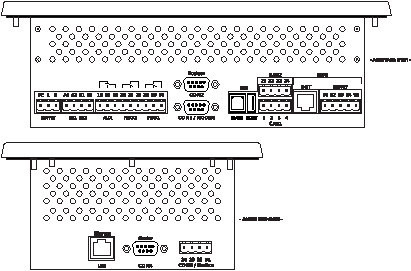
\includegraphics[scale=0.54]{images/CI4000_Hardware.pdf}
\caption{Schittstellen Marktrechner}
\label{fig:marktrechner_interfaces}
\end{figure}

Das Betriebssystem auf dem Marktrechner ist eine eigene Linux-Distribution, welche mit der Software ptxdist, der  Pengutronix e.K., erstellt wird. Ptxdist bringt einige Hundert Module und Bibliotheken mit, welche über einen einfachen Dialog an- und abgewählt werden können. Mit ein wenig Konfigurationsaufwand können auch eigene Module mit aufgenommen werden. Dadurch kann eine sehr schlanken Distribution erzeugt werden, die  auf den eigenen Software-Stack zugeschnitten ist. Die eigenen Softwaremodule sind in C++ und dem Qt-Framework geschrieben. 

\paragraph{Architektur}

Alle Daten und Meldungen, die der Marktrechner sammelt und aufbereitet, müssen zu einem Zeitpunkt von einem Menschen ausgewertet werden. Die 24-Stunden Überwachung vor Ort, durch einen Mitarbeiter, ist nicht wirtschaftlich. Deshalb übernehmen heutzutage großteils Fernservice-Zentralen (FSZs) die Überwachung von Kälteanlagen. Der Marktrechner kann aus der Ferne über eine Ethernet- oder Modem-Verbindung erreicht werden. Letztere wird, aufgrund ihres aussterbendes Charakters, an dieser Stelle nicht weiter erläutert. Für den Zugriff auf die Ethernet-Schnittstelle sind Fernservice-Zentralen, über VPN, mit einem oder mehreren Unternehmensnetzwerken, ihrer Kunden, verbunden (Abbildung~\ref{fig:current_setup}). Über dieses können die Marktrechner erreicht werden. Auf diese Weise kann eine einzige Fernservice-Zentrale Tausende Marktrechner überwachen. Der Marktrechner fungiert als Server, das heißt Daten und Meldungen müssen aktiv von einer Fernservice-Zentrale abgeholt werden. Ist aus den abgeholten Daten ersichtlich, dass ein Fehler in der Anlage aufgetreten ist, kann die Fernservice-Zentrale entweder direkt eingreifen oder einen Monteur zum betreffenden Kunden schicken, der die Anlage instand setzt.

\begin{comment}
@startuml images/problemfeld.svg
skinparam monochrome true
skinparam dpi 150

package "Unternehmensnetzwerk A" as UA {
  [Marktrechner 1]
  [Marktrechner 2]
  [...]
  [Marktrechner n]
}

package "Unternehmensnetzwerk B" as UB {
}

package "Unternehmensnetzwerk C" as UC {
}

cloud VPN {
}

[Fernservice-Zentrale] -down- VPN
VPN -down- UA
VPN -left- UB
VPN -right- UC
UA - [Marktrechner n]
UA - [...]
UA - [Marktrechner 2]
UA - [Marktrechner 1]

@enduml
\end{comment}

\begin{figure}[h]
\centering
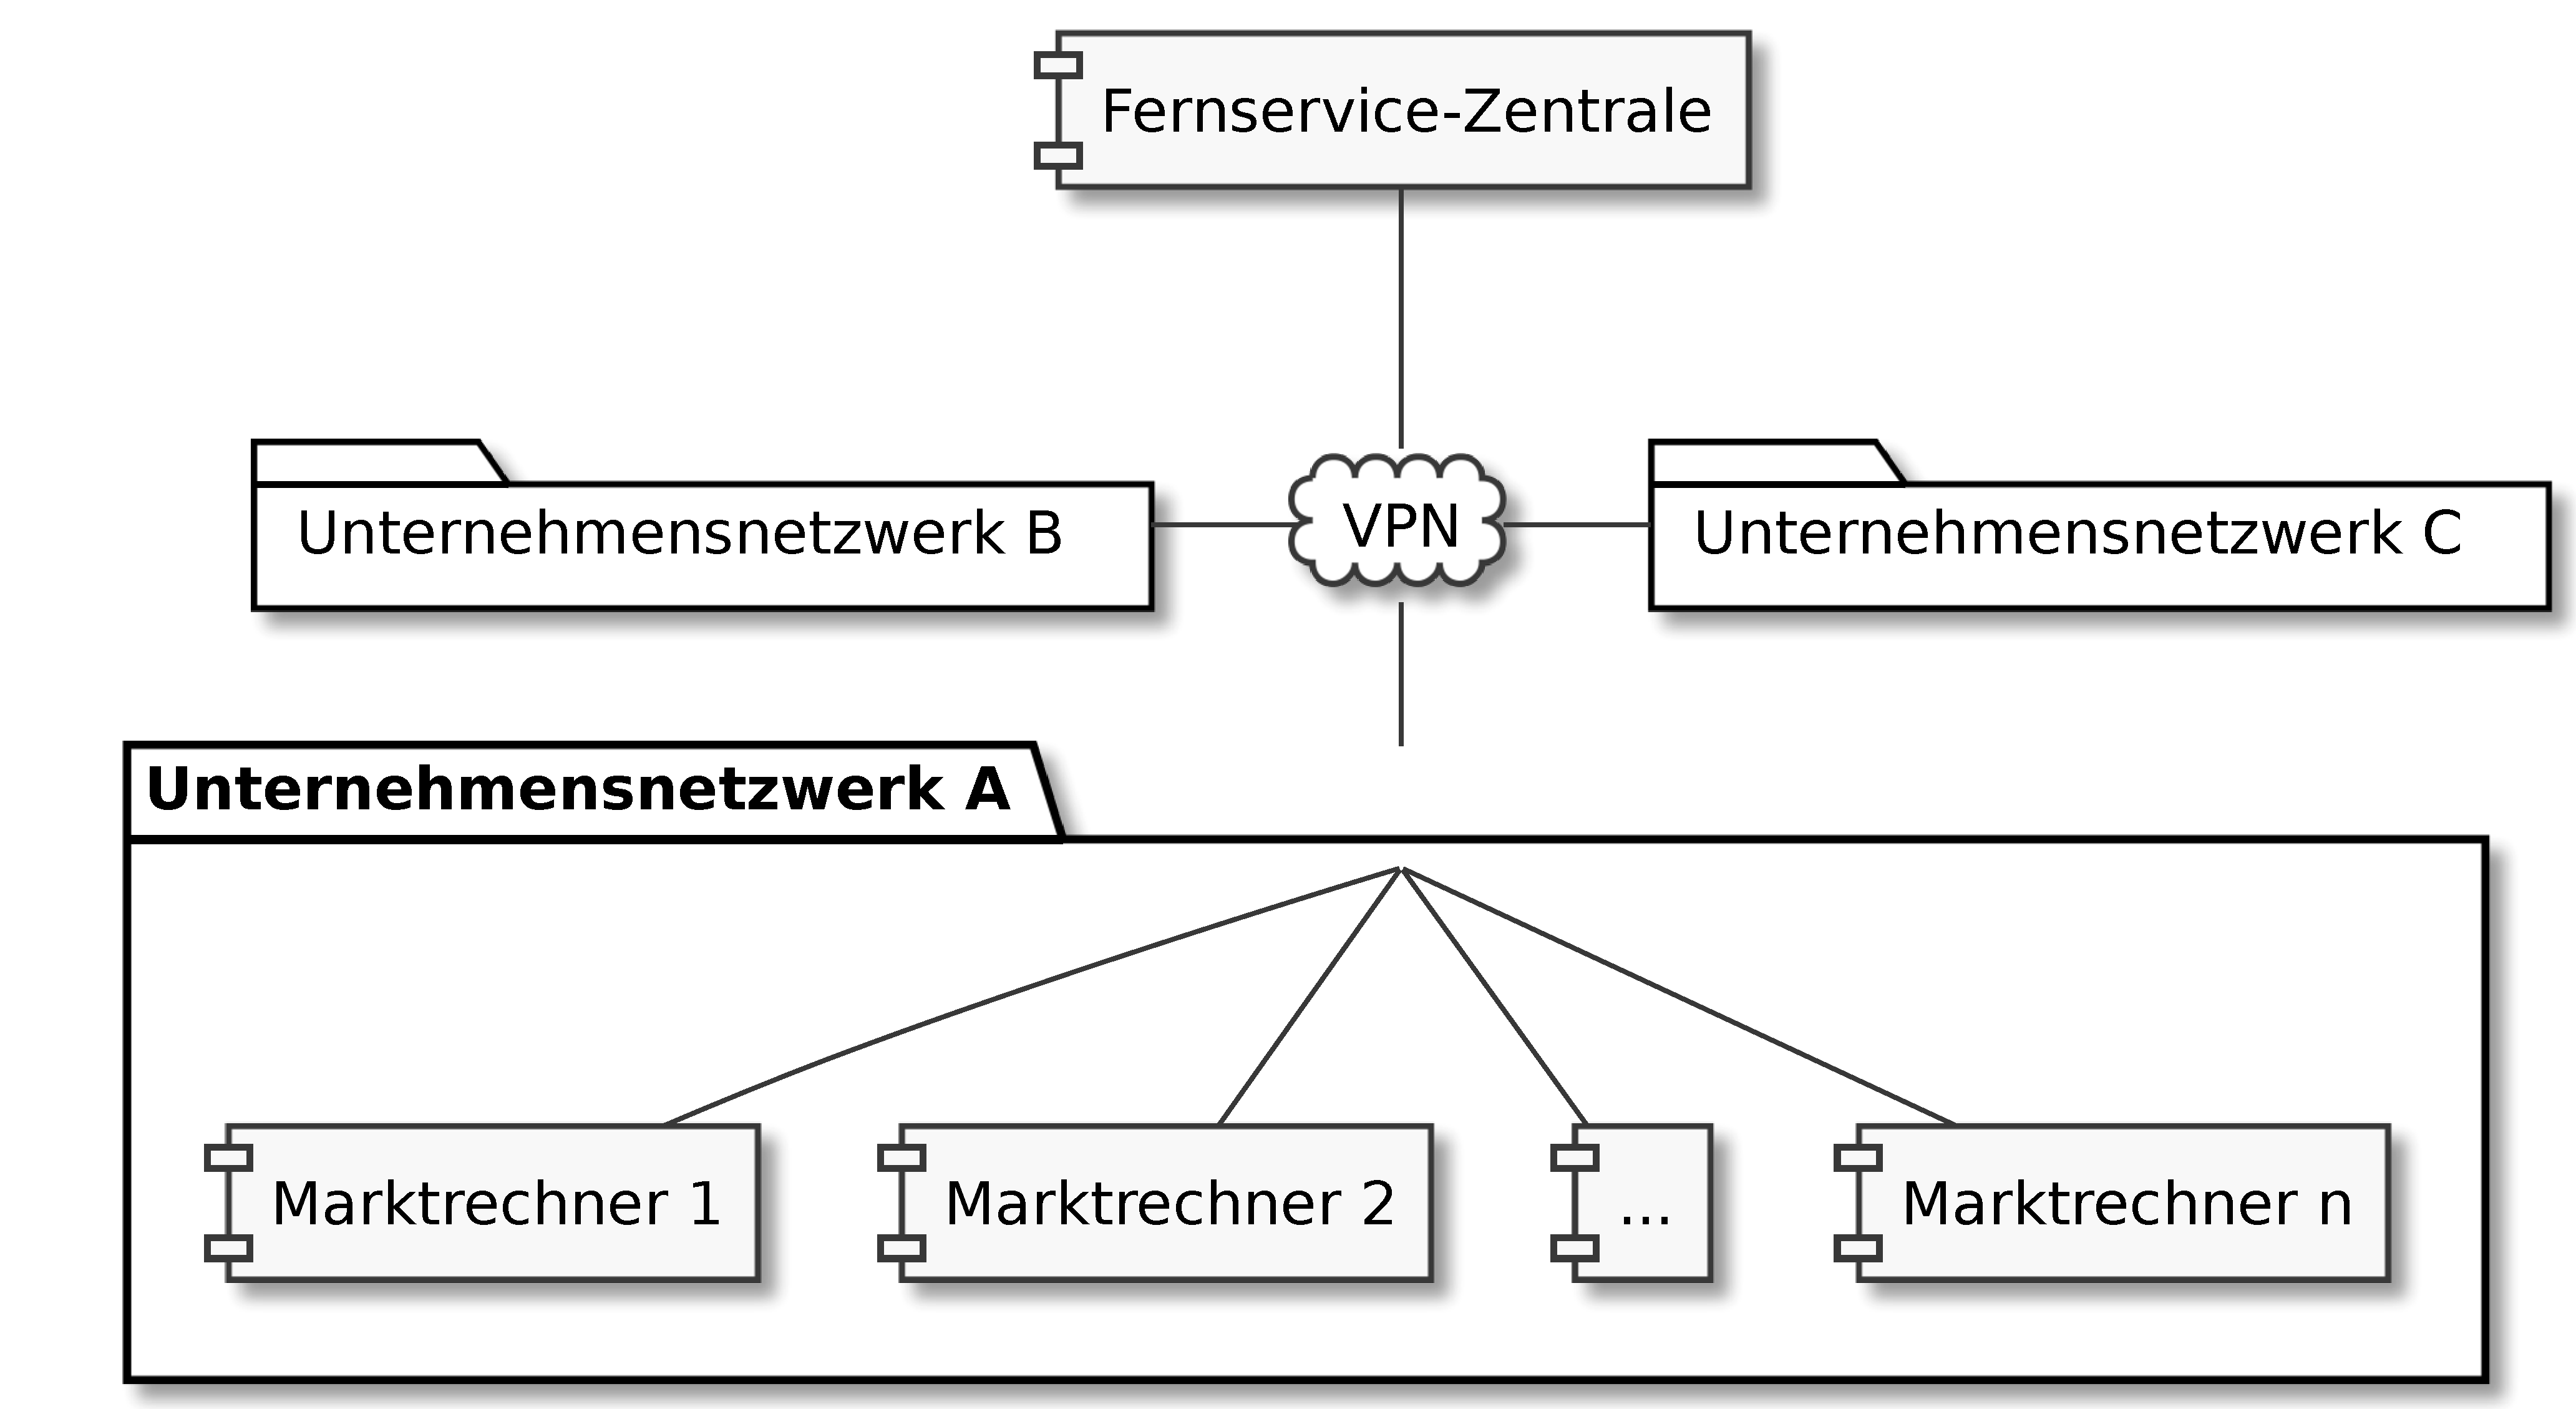
\includegraphics[scale=0.2]{images/problemfeld.pdf}
\caption{Aktuelle Vernetzung}
\label{fig:current_setup}
\end{figure}

Beim Einsatz von VPN ist die Kommunikation von der Fernservice-Zentrale bis zum Unternehmensnetzwerk abgesichert. Im Lokal Area Network (LAN) des Unternehmens ist der gesamte Datenverkehr zu und von den Marktrechnern allerdings unverschlüsselt. Es gibt zwei Arten von Datenverkehr zum Marktrechner, zum einen über das proprietäre Protokoll des Herstellers und zum anderen über Webservices auf Basis von einfachen XML-RPCs. Ein Angreifer, mit Zugriff auf das LAN und Kenntnisse des Hersteller-Protokolls, hätte die Möglichkeit den Datenverkehr zwischen Fernservice-Zentrale und Marktrechner mitzulesen. Viel schwerwiegender als das mitlesen der Kommunikation ist, dass ein solcher Angreifer über das Protokoll vollen lesenden und schreibenden Zugriff auf das System erhalten kann, da es keine geeignete Autorisierung und Authentifizierung gibt. Die Anzahl an Personen mit Wissen über das Hersteller-Protokoll schränkt allerdings den Kreis der möglich Angreifer ein. Viel wahrscheinlicher ist ein Angreifer, mit Zugriff auf das LAN ohne Kenntnisse des Hersteller-Protokolls. Dieser kann den Datenverkehr zwischen XML-RPC und Fernservice-Zentrale mithören. Da in der XML die Daten interpretierbar aufbereitet wurden ist es ein leichtes diese Daten auszuwerten. Auch hier sind keine geeignete Autorisierungs- und Authentifizierungstechniken eingesetzt, wodurch der Angreifer statt mitzulesen, den XML-RPC selbst befragen könnte. Dadurch erlangt er zwar keine vollen Zugriff auf das System, kann jedoch einige wichtige Schnittstellen auslesen und zum Teil auch neu konfigurieren. 

Neben diesen offensichtlichen gibt es weitere Mängeln. Zum Beispiel sind aussagekräftige Logs Hauptbestandteil eines guten Systems. Sinnvoll ist das protokollieren des Systemzugriffs. Durch die ungeeigneten Sicherheitsmaßnahmen verliert das Zugriffslog jedoch komplett an Aussagekraft und ist damit wertlos. Ein weiterer Mangel ist, dass der Hersteller durch die existierende End-to-Site VPN-Verbindung keinen Zugriff auf die Systeme erlangen kann, um Unterstützung bei Problemen zu leisten. 

\subsection{Alarmmanagement} beschreibt Tätigkeiten, um die Alarmierung einer Kälteanlage. Dazu gehört in ersten Schritt das Anlegen und das Konfigurieren der Alarme. Als nächstes sieht es die aktive, durch Polling am System, oder passive, durch Pushen des Systems, Versand der Alarme vor. Außerdem beinhaltet es das Auswerten archivierter Alarme. Ein Alarm trifft eine Aussage über den Betriebszustand der Kälteanlage. Beispielsweise, wird ein Alarm ausgelöst, wenn die Temperatur in einen Kühlgerät für die darin gelagerte Waren einen bestimmten Grenzwert übersteigt.

\subsection{Offline-Konfiguration} Eine an den Markt angepasste Konfiguration der Kälteanlage, welche vor Inbetriebnahme erstellt wurde. Ein Teil ist die genaue Parametrierung der Kühlgeräte und Kühlmöbel, unter Berücksichtigung der darin zu lagernden Ware.

\section{Sicherheitskonzept}

Viele Sicherheitssysteme heutzutage sind 'sicher', da niemand sich die Mühe gemacht hat, diese anzugreifen \cite{gutmann0}. Ein Großteil an Problemen von Sicherheitskonzepten entsteht, weil Sicherheit im Nachhinein angeheftet wird, ohne sich die Mühe zu machen das Gesamtsystem zu betrachten. Bevor man über potentielle Eigenschaften eines Sicherheitssystems nachdenkt muss man zunächst die Umgebung betrachten, in welcher das System eingesetzt werden soll \cite{gutmann4}. Wenn heutzutage über Sicherheit diskutiert wird, wird meistens ausschließlich über Kryptographie gesprochenen. Auch wenn Kryptographie Hauptbestandteil jedes Sicherheitssystems ist, ignorieren praktisch alle Angriffe auf ein Sicherheitssystem die Kryptographie und attackieren den Weg wie es genutzt wird \cite{gutmann1}. Ein bekanntes Beispiel hierfür ist der Heartbleed-Bug\footnote{http://heartbleed.com/}, der eine Lücke in der Heartbeat-Implementierung, der OpenSSL Bibliothek, ausnutzt, um sich Zugriff auf den Privaten Kommunikationsschlüssel zu verschaffen. Es macht also wenig Sinn utopisch lange Schlüssel zu nutzen, wenn kein Angreifer sich darum schert. Zudem wird durch Verschlüsselung das Hauptproblem eines Sicherheitssystems 'Vertrauen' unzureichend betrachtet. Vertrauen wird geschaffen durch Authentifizieren. Drei beliebte Konzepte für die Authentifizieren sind Passwörter, Pre-Shared-Keys (PSK) und Public-Key-Verfahren. Passwörter haben das Problem, dass sie einen Teil der Sicherheit auf den Benutzer abgehen, indem angenommen wird, dass Benutzer immer sichere Passwörter wählen. Da dies in der Realität nicht so ist wird versucht mit absurden Passwortregeln Benutzer zu zwingen Passwörter zu wählen, die Sie sich nicht merken können. Hierbei sollte beachtet werden das Benutzer Sicherheit lieber ausschalten oder umgehen als sich damit auseinanderzusetzen \cite{gutmann5}. Darüber hinaus können Passwörter lediglich einseitige Authentifizieren schaffen, wie etwa eine Anmeldung bei einem E-Mail Provider. Durch Angabe des Passwort weiß der Server, welchem Client er vor sich hat und kann diesem bestimmte Mails anvertrauen. Der Client kann nur die Domain überprüfen und hoffen, dass diese korrekt aufgelöst wird. Zwar versucht man über Zertifikate und Zertifikat-Autoritäten Vertrauen aufzubauen, aber das einzige was ein Zertifikat bescheinigt ist der Geldaustausch zwischen dem Zertifikat-Halter und der Zertifikat-Autorität, keinesfalls aber das dessen Identität geprüft wurde, was Vertrauen schaffen könnte. Vertrauen kann nur durch eine Identitätsprüfung geschaffen werden \cite{gutmann8}. Beim Austausch von PSKs geschieht dies Implizit. Bei PSKs wird eine Austauschkanal benötigt, der nicht der unsichere Kommunikationskanal ist, zum Beispiel über den traditionellen Postweg. Dadurch das man darauf vertraut, dass die Post den Schlüssel nur dem Empfänger übergibt, kann man hier Vertrauen aufbauen. Bei Public-Key Verfahren hat man den Austauschkanal eliminiert, da die Schlüssel ohne Probleme über einen unsicheren Kanal getauscht werden können. Allerdings hat man dadurch das Verlangen nach einen Authentifizierungskanal geschaffen. Das Problem, dass für die Authentifizierung zwingen ein zweiter Kommunikationskanal benötigt wird, besteht bis heute ohne das es eine geeignete Lösung dafür gibt. 

Als Teil des Sicherheitskonzeptes dieser Arbeit wird es sein dieses Authentifizierungsproblem auf geeignete Weise zu berücksichtigen, ohne das durch den Einsatz einer bestimmten Technologie im Extremfall enorme Kosten entstehen können. 


\chapter{Bedrohungsmodell} \label{chap:threat}
\epigraphhead[70]{\epigraph{The only truly secure system is one that is powered off, cast in a block of concrete and sealed in a lead-lined room with armed guards.}{\textit{Gene Spafford}}}

Das Bedrohungsmodell soll auf mögliche Gefährdungen des aktuellen Systems hinweisen. Diese werden analysiert und schrittweise, durch geeignete Maßnahmen, versucht einzudämmen. Eine aussagekräftige Analyse setzt die Wahl eines geeigneten Modells voraus. 

\section{Modellübersicht}

Die beiden Modelle die erläutert und gegenübergestellt werden sind, der IT-Grundschutz und die Soft Systems Methodology (SSM). Während der IT-Grundschutz auf Sicherheitssysteme spezialisiert ist, lässt sich SSM auch allgemein verwenden.

\subsection{BSI Sicherheitskonzept}
Folgende Ausführungen sind dem BSI IT-Grundschutz Empfehlungen entnommen \cite{bsi_standard1,bsi_standard2,bsi_standard3,bsi_standard4}.
Das Bundesamt für Sicherheit in der Informationstechnik stellt im Rahmen seiner IT-Grundschutz Empfehlungen auch ein Modell zur Entwicklung von Sicherheitskonzepten dar. In Abbildung~\ref{fig:bsi_sicherheit} sind die empfohlenen Schritte gezeigt. Das Modell des BSI betrachtet ein Sicherheitskonzept rein aus technischer Seite und nimmt direkten Bezug auf die Reale Welt. Schritt eins, verlangt die Erfassung aller Komponenten im Geltungsbereich. Dazu soll das Zusammenspiel zwischen Geschäftsprozessen und Anwendungen herausgearbeitet werden. Als nächstes soll der Schutzbedarf, der Komponenten aus Schritt eins, ermittelt werden. Der ermittelte Schutz soll gemäß der eingesetzte Informationstechnik ausreichend beziehungsweise angemessen sein. Anhand dieser Informationen werden, für die Zielobjekte aus Strukturanalyse und Schutzbedarf, Bausteine aus dem IT-Grundschutz gewählt. Der anschließende Basis-Sicherheitscheck soll das aktuelle Sicherheitsniveau einschätzen und liefert als Ergebnis eine Liste der relevanten Maßnahmen und ihrem Umsetzungsstatus "entbehrlich", "ja", "teilweise" oder "nein". Dafür sollen Gefährdungenkataloge und Maßnahmenkataloge des BSI genutzt werden. In Schritt vier wird geprüft, ob die Standard-Sicherheitsmaßnahmen ausreichend sind, was für die meisten typischen Geschäftsfelder der Fall seinen sollte. Sollten erweitere Sicherheitsmaßnahmen nötig werden muss für diese eine Risikoanylse durchgeführt werden. Bei den Standard-Sicherheitsmaßnahmen ist dies bereits durch die IT-Grundschutz-Kataloge abgedeckt. 

\begin{figure}[htbp]
\centering
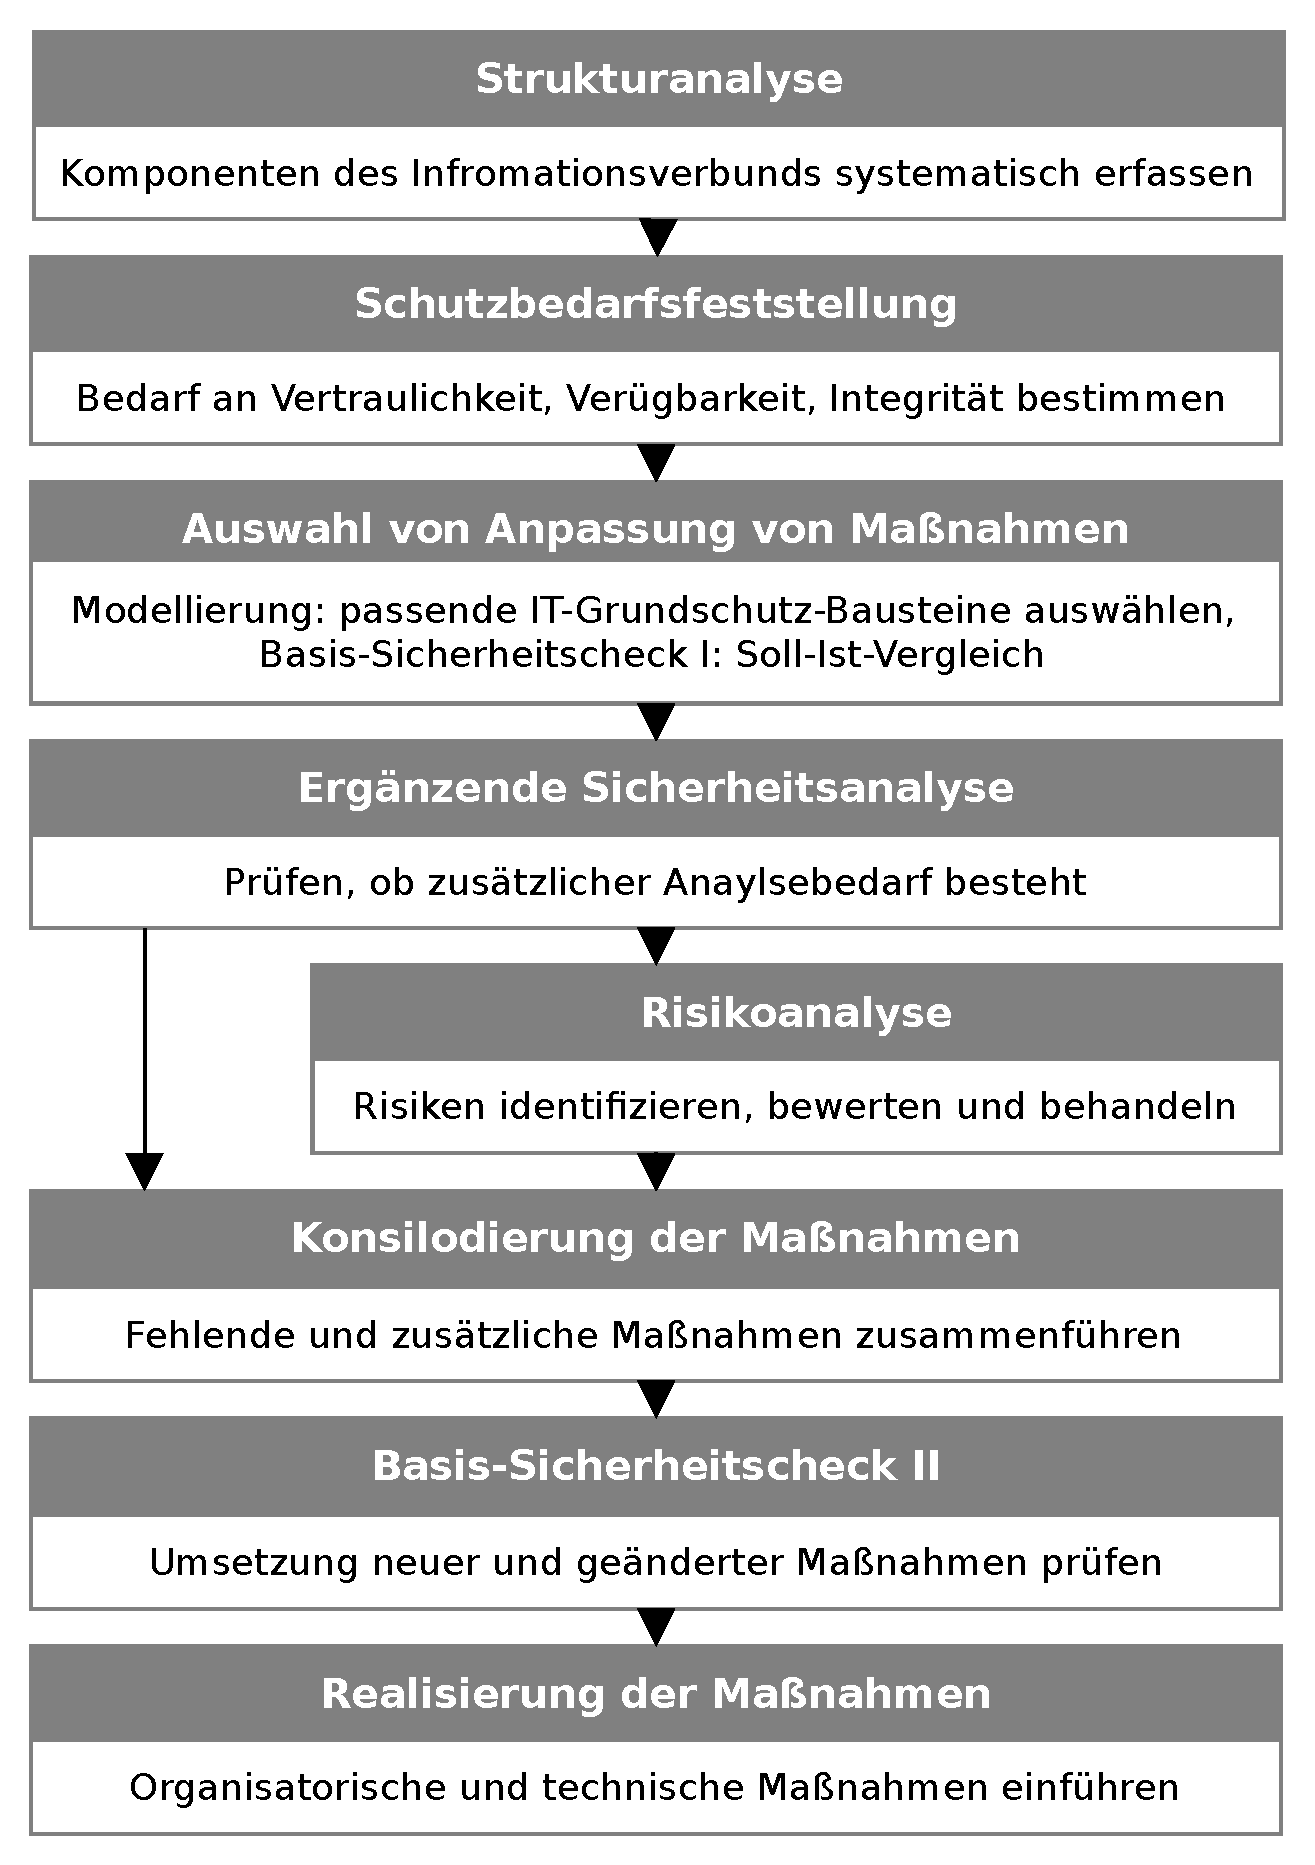
\includegraphics[scale=0.35]{images/bsi_sicherheitskonzept.pdf}
\caption[BSI Sicherheitskonzept]{BSI Sicherheitskonzept\footnotemark}
\label{fig:bsi_sicherheit}
\end{figure}
\footnotetext{Der Zeichnung \cite{bsi_img} des BSI nachempfunden, aufgrund unangemessener Bildqualität}

Ab Schritt sechs erfolgt die Durchführung der Maßnahmen. Bei der Konsolidierung wird geprüft, welche Maßnahmen aus den IT-Grundschutz-Katalogen tatsächlich, in der Praxis, umsetzbar sind. Teilweise müssen einige Maßnahmen noch an Begebenheiten im Unternehmen angepasst werden. Unter Berücksichtigung des verfügbaren Budgets und des verfügbaren Personals, werden die entsprechenden Maßnahmen für die Umsetzung geplant. Im zweiten Sicherheitscheck wird abschließend ein erneuter Soll-Ist-Vergleich durchgeführt, um die Ergebnisse der Maßnahmen zu überprüfen. Als letzter Schritt werden die Maßnahmen im Alltagsgeschäft in Betrieb genommen.

\subsection{Soft Systems Methodology}

Eine geeignete Analyse- und Designmethodik für ein Bedrohungsmodell, bietet die Soft Systems Methodology (SSM), Abbildung~\ref{fig:ssm}.

\begin{figure}[htbp]
\centering
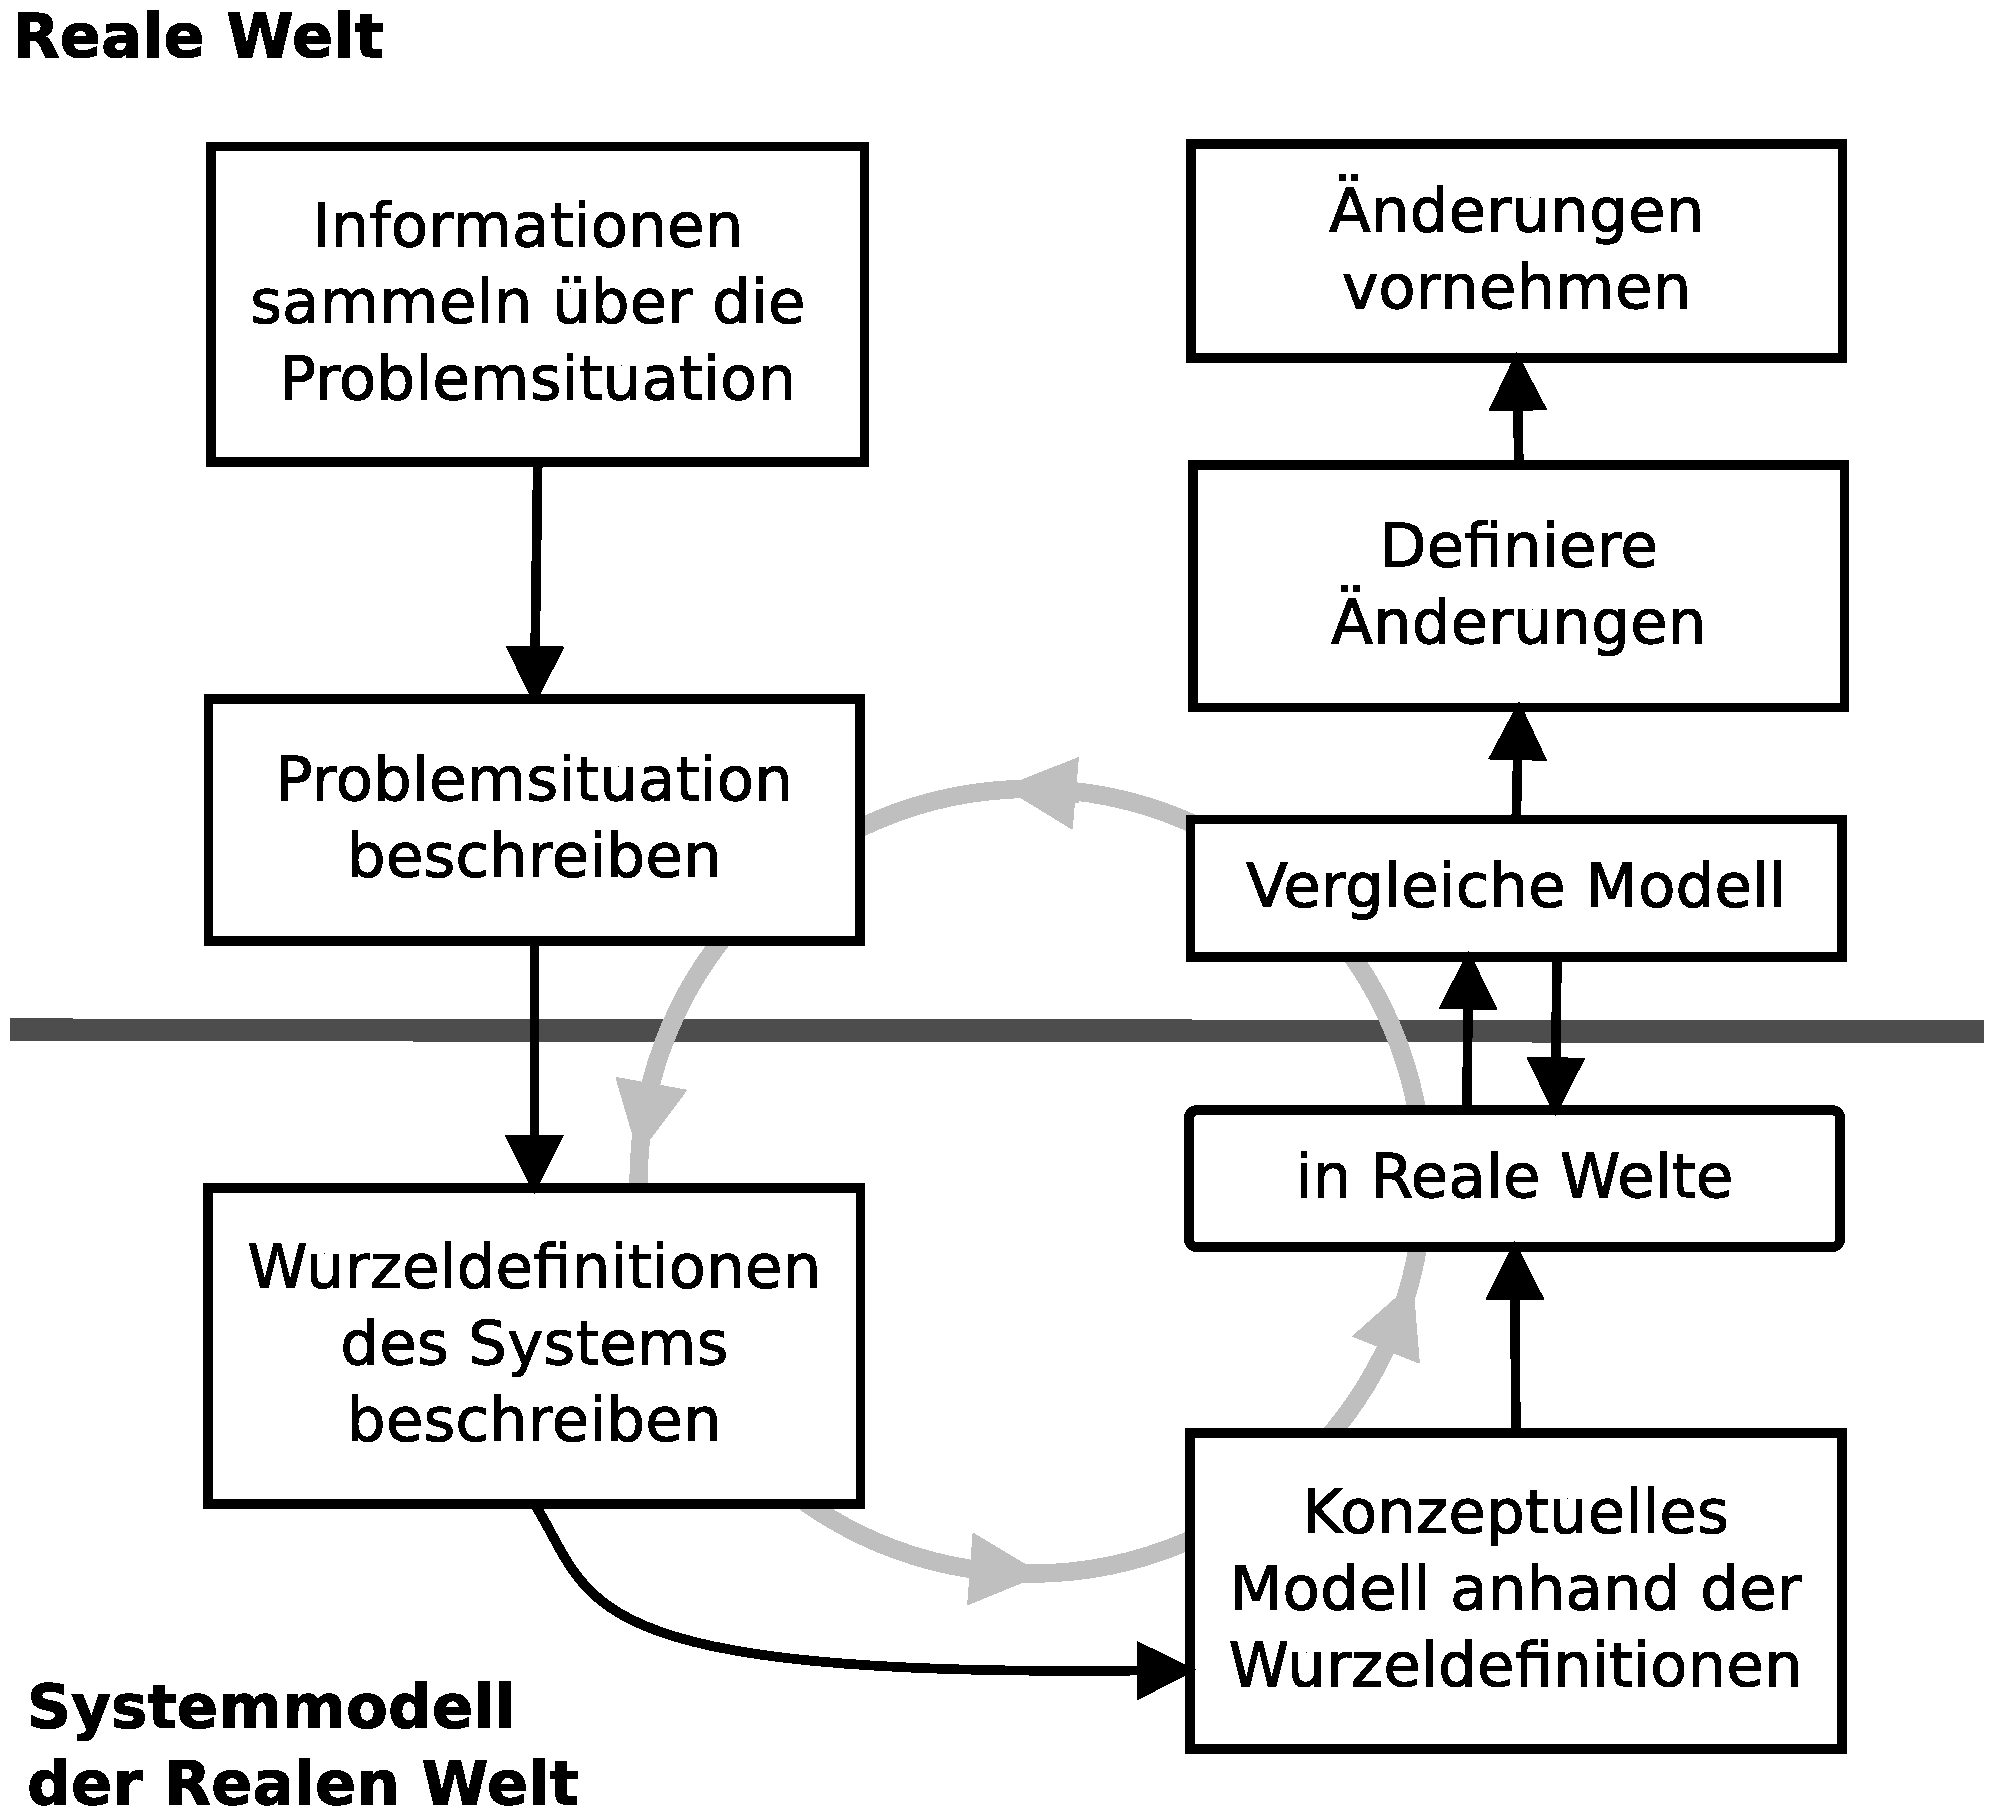
\includegraphics[scale=0.30]{images/ssm.pdf}
\caption{Soft Systems Methodologie}
\label{fig:ssm}
\end{figure}

SSM wurde in den späten 1960er Jahren, an Universität von Lancaster, von Peter Checkland, begonnen zu entwickeln. Es war zunächst als Modellierungswerkzeug gedacht, wird aber hauptsächlich als Lern- und Bedeutungswerkzeug angesehen \cite{bobwill}. SSM kann prinzipielle immer dann eingesetzt werden, wenn jemand versucht zielgerichtet zu handeln \cite{checkland1}. Ein wichtiger Teil von SSM ist die Weltansicht, welche einem Vorgehen Sinn und Zweck verleiht. Beispielsweise, des einen Terrorist ist des anderen Freiheitskämpfer. Beide betrachten jedoch das Selbe. Durch mehrere zielgerichtete Vorgehen, unterschiedlicher Weltansichten, wird in SSM versucht die Reale Welt zu beschrieben. Diese ist jedoch viel zu komplex, um in irgendeiner Modellsprache erfasst zu werden. Daher wird das Vorgehen bewusst auf ein rein konzeptionelles Modell beschränkt. Diese Einschränkung verringert die Komplexität und soll dadurch die Problemlösung vereinfachen. Die Trennung zwischen Realer Welt und Systemabbild der Realen Welt findet im Modell zwischen Phase 1 und 2 statt. In der ersten Phase wird die gesamte Problemsituation der Realen Welt, aus Sicht aller Beteiligten, erörtert und unstrukturiert beschrieben. Anhand dieser Informationen werden in der zweiten Phase, die bereits genannten, konzeptuellen Modelle erstellt. Die Modelle dienen dazu Debatten über die Thematik zu strukturieren, indem Sie mit der Realen Welt verglichen werden. In einem iterativen Prozess werden die ersten beiden Phasen wiederholt, bis die Thematik klar genug ist Ergebnisse zu treffen. Die Ergebnisse werden anschließend in konkrete Schritte formuliert, die ausgeführt werden sollen.

Im Kontext des Bedrohungsmodell wird SSM eingesetzt, um das zielgerichtete Vorgehen ein Sicherheitskonzept zu erstellen zu analysieren. Die unterschiedlichen Weltansichten entstammen der Betrachtung eines Beschützers und Angreifers des Systems. Anhand deren konzeptionellen Modelle soll möglichst ganzheitliches Bedrohungsbild entstehen, aus welchem konkrete Schritte abgeleitet werden können.

\subsection{Modellentscheidung}

Das vom BSI vorgeschlagene Konzept betrachtet aus technischer Sicht alle Aspekte, welche ein Sicherheitsmodell umfassen sollte. Vom Konzept her ist es jedoch wesentlich zu komplex, da es für Sicherheitskonzepte kompletter Unternehmen ausgelegt ist, die eine teure Zertifizierung, als "Qualitätsmerkmal", durch den BSI anstreben. Zudem nimmt die vom BSI vorgeschlagenen Vorgehensweise keinerlei Rücksicht auf verschiedene Weltanschauungen. Im Bezug auf die Bedrohungsanalyse, kann diese allenfalls aus der Weltanschauung des Unternehmens komplett sein. Die Soft Systems Methodology ist zwar nicht als Methodik zur Erstellung eines Sicherheitskonzeptes gedacht, dennoch ist sie als Vorgehensweise durch ihre Trennung zwischen Realer Welt und deren Abstraktion besser geeignet. Im Gegensatz zum Vorgehen des BSI wird nicht alles anhand großer Tabellen stur abgearbeitet, SSM wurde geschaffen, um Einfluss auf das menschliche Denken und Vorgehen zu nehmen und soll diese zu optimieren. Das heißt nicht, dass alles aus dem IT-Grundschutz des BSI unbrauchbar, für anwendungsspezifische Sicherheitskonzepte, ist. Unter anderem die Vorarbeit, die der BSI mit Gefährdungenkataloge und Maßnahmenkataloge geleistet hat lässt sich auch mit SSM verwenden.

\section{Beschreibung der Problemsituation} \label{sec:problem_situation}

Die in Abschnitt~\ref{sec:marktrechner} geschilderte Architektur des Marktrechnerumfeldes, zeigt einige Mängel des aktuellen Systems auf. Die Abbildung~\ref{fig:current_setup} zeigt ein unstrukturiertes Bild, in SSM Terminologie Rich-Picture. Es ist wichtiges Hilfsmittel zur Beschreibung der Problemsituation, welches möglichst viele Informationen in einem Bild erfassen soll. Besonders Grenzen, Struktur, Informationsflüsse, Kommunikationskanäle und das menschliche Aktivitätssystem sollen aufzeigt werden \cite{ssmger}. Der Fokus dieser Arbeit liegt auf dem Fernzugriff, dennoch werden auch die Probleme des lokalen Zugriffes erfasst. Dadurch soll verhindert werden, dass der Fernzugriff unnötige Hindernisse für die lokale Zugriffskontrolle schafft. 

\begin{figure}[h]
\centering
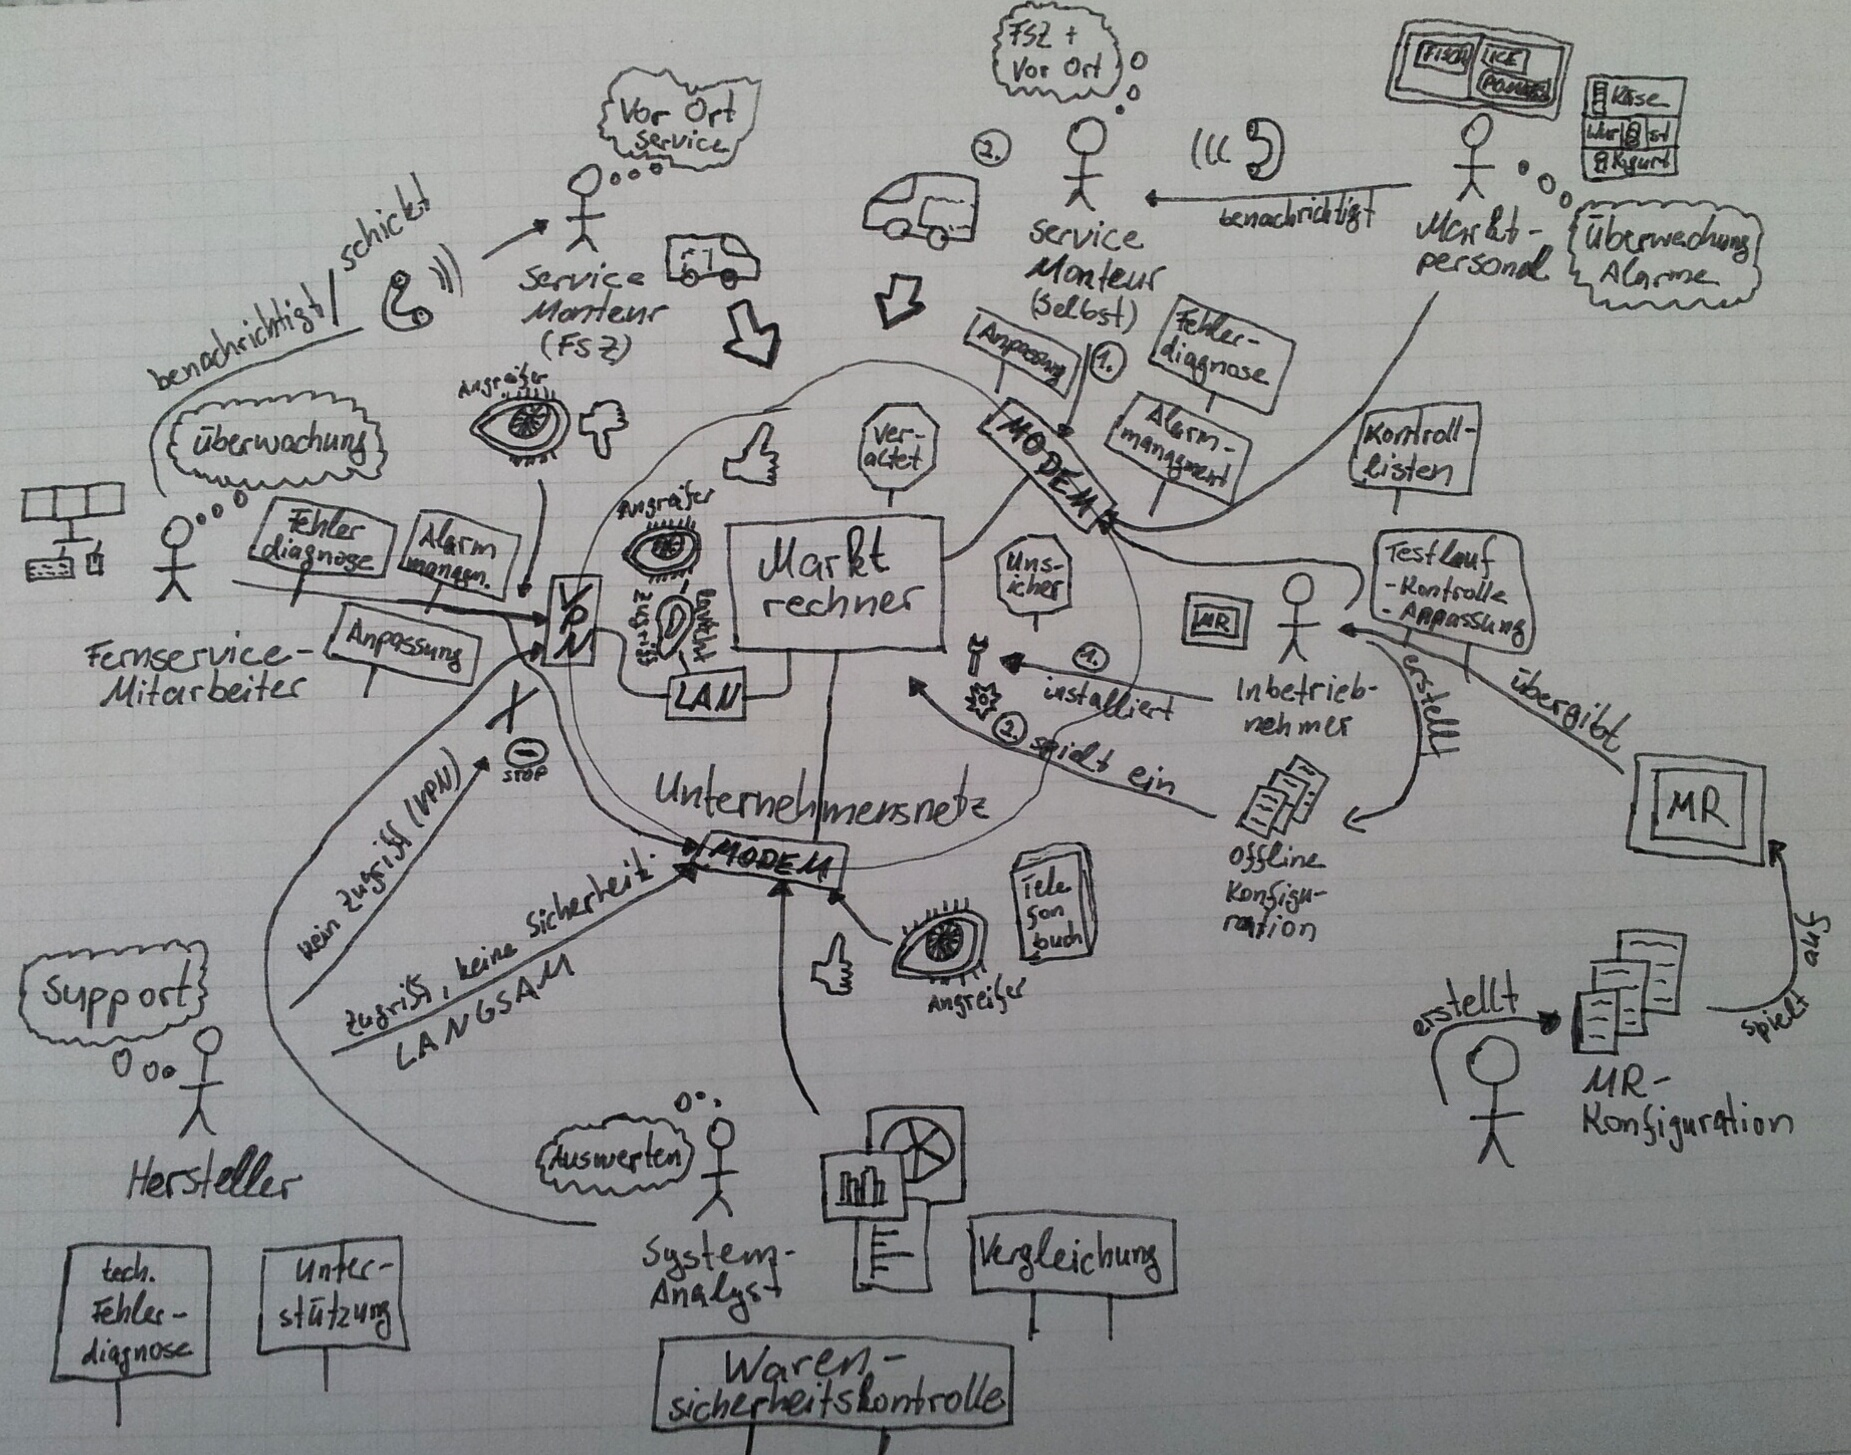
\includegraphics[scale=0.237]{images/problemsituation.jpg}
\caption{Problemsituation}
\label{fig:current_setup}
\end{figure}

\subsection{Identifizieren der Rollen} \label{sec:roles}

Zunächst wird ein Überblick über alle Zugriffsberechtigten geschafft. Diese werden anhand von Rollen zusammengefasst, welche Funktion und Zugriffsart beschreiben. Es ist durchaus möglich, dass ein Zugriffsberechtigter mehrere Rollen annehmen kann. Alle Rollen sind in der Abbildung~\ref{fig:current_setup} illustriert. Die Beschreibungen der Rollen sind allgemein gehalten und nehmen keinen Bezug aktuelle oder zukünftige technologische Begebenheiten.

\paragraph{Der Inbetriebnehmer} ist die Rolle, welche das System initial zum Laufen bringt. Der Inbetriebnehmer muss lokal, vor Ort die Anlage in Betrieb nehmen. Dazu kann er bereits im Voraus eine Offline-Konfiguration anlegen, welche an die Anlage des Kunden angepasst ist. Die Konfiguration wird auf die Anlage eingespielt, sobald die Hardware installiert ist. Bevor die Anlage produktiv eingesetzt werden kann, wird ein Testlauf durchgeführt. Während des Testlaufs muss der Inbetriebnehmer die Anlage überwachen, um bei Problemen die Konfiguration, die Parameter und die Einstellungen anzupassen. Zur Überwachung des Testlaufes muss der Inbetriebnehmer nicht zwingend vor Ort sein, sondern kann den Status auch aus der Ferne abrufen, damit der Inbetriebnehmer nicht etliche Stunden neben dem Marktrechner auf das Auftreten von Fehlern warten muss.
\paragraph{Der Projektierer} konzipiert und entwirft komplette Kälteanlagen. Ein Teil seiner Aufgaben kann sein die Offline-Konfiguration erstellen. Diese kann dann direkt von Werk aus aufgespielt werden. Der Inbetriebnehmer muss den vorkonfigurieren Marktrechner dann lediglich noch installieren und testen.
\paragraph{Der Service-Monteur} führt Wartungen und Störungsbehebungen durch. Für den Service-Monteur gibt es zwei denkbare Ausprägungen. Als Selbständiger wird er im Fall einer Störung, durch den Eigentümer der Anlage oder dessen Personal, benachrichtigt. Nun hat er die Möglichkeit aus der Ferne eine Fehlerdiagnose durchzuführen und Veränderungen an der Konfiguration und dem Alarmmanagement durchzuführen. Sollte er nicht in der Lage sein die Störung aus der Ferne zu beheben muss er die selben Tätigkeiten vor Ort durchführen können. Als Angestellter einer Fernservice-Zentrale entfällt die Diagnose und die Fehlerbehebung aus der Ferne, da dies bereits durch Mitarbeiter der FSZ durchgeführt wurde. Wenn die Störung von dort nicht gelöst werden kann, wird der Service-Monteur zur Anlage geschickt.
\paragraph{Der Fernservice-Mitarbeiter} überwacht mehrere Anlagen aus der Ferne. Diese Rolle führt die selben Tätigkeiten wie ein Service-Monteur durch. Allerdings erfolgt bereits erwähnte Fehlerdiagnose, Kontrolle und Anpassung von Parametern und Einstellungen, sowie das Alarm-Management ausschließlich aus der Ferne. Einige Störungen können durch anpassen der Konfiguration hinausgezögert werden bis ein Service-Monteur vor Ort ist. Dadurch kann zum Beispiel Warenschaden auf Kosten von Energieeffizienz verhindern werden.
\paragraph{Der System-Analyst} wertet relevante und vergleichbare Daten zur Energieeffizienz und Warensicherheit aus. Auch er arbeitet ausschließlich aus der Ferne. Auswertbare Daten sind etwa Temperaturwerte oder Energieverbrauch. Sollten diese Werte im Vergleich mit anderen Anlagen negativ auffallen, kann er veranlassen, dass eine Anlage überprüft wird.
\paragraph{Das Eigentümer/Marktpersonal} ist daran interessiert eine Kontrolle der Parameter zur Warensicherheit durchzuführen und eine Dokumentationen der Waren-Temperaturen zu erhalten. Auch soll das Marktpersonal über Alarme informiert werden, um einen Service-Monteur zu benachrichtigen und Warenschaden zu verhindern. Die Rolle des Marktpersonal kann Zugriff vor Ort benötigen, aber auch der Zugriff aus der Firmenzentrale wäre denkbar.
\paragraph{Der Hersteller} ist eine weitere exklusiv aus der Ferne agierende Rolle. Er soll anderen Rollen Unterstützung bei ihren Arbeiten leisten können. Vor allem bei Softwareproblemen sind Monteure nicht in der Lage das Problem an der Anlage alleine zu beheben.
\paragraph{Fremdsysteme} ...


\subsection{Systemumgebung}

Der Fernzugriff auf einen Marktrechner ist prinzipielle immer möglich. Zwei Arten des Fernzugriffs sind etabliert, über VPN oder Modem. Verbindungen über VPN kommen nur in Fernwarten zum Einsatz. Etwa die Hälfte der Marktrechner können auf diese Weise erreicht werden. Der Einsatz von VPN hat den Nachteil, dass er extrem aufwendig zu etablieren ist. Denn hier treffen unterschiedliche IT-Infrastrukturen zusammen, was ein Garant für Probleme ist. Überschneidungen bei IPv4-Adressen ist dabei nur ein Beispiel. Außerdem beschränkt sich der Zugriff ausschließlich auf die gekoppelten Netze. Dadurch ist es dem Hersteller nicht möglich Unterstützung, aus der Ferne, zu leisten. Alle anderen Verbindungen werden über Modems ermöglicht. Deren Einsatz ist veraltet und bietet nur sehr geringe Übertragungsgeschwindigkeiten. Zudem stellen immer mehr Internet-Provider analoge ISDN-Anschlüsse auf Voice-over-IP (VoIP) Lösungen um. VoIP sorgt allerdings dafür, dass eine zuverlässige Modem-Kommunikation unmöglich wird. Für einen Angreifer ergeben sich bei den Verbindungen drei Angriffsvektoren. Über VPN ist die Verbindung bis zum Unternehmensnetz gesichert. Innerhalb des LAN hat ein Angreifer freies Spiel. Auch die Modem-Verbindung stellt für einen Angreifer kein Hindernis dar, da er lediglich die Telefonnummer kennen muss. Zusätzlich kann er die Modem-Leitung dauerhaft blockieren und dadurch unterbinden das Anderen zugriffen können.

\begin{comment}
Die genannten Rollen müssen nun in die Systemumgebung eingeordnet werden. Der Marktrechner wird als Teil einer Kälteanlage beim Kunden installiert. Dort wird er an das Netzwerk des Unternehmens angeschlossen. Die lokale Bedienung ist auf geeignete Weise abgesichert, um herumspielen mit der Anlage zu unterbinden. Das hacken des lokalen Zugriffs ist sehr unwahrscheinlich, da jemand mit Zugriff auf den Marktrechner ebenfalls Zugriff auf die Kälteanlage hat und dort physikalisch deutlich leichter Schaden anrichten kann. Aus der Ferne muss der Marktrechner für die Fernservice-Zentrale und für den Hersteller erreichbar sein. Beide befinden sich an unterschiedlichen geographischen Standorten. Optional kann der Zugriff anderer Fernzugriffe, an anderen Standorten, erlaubt werden. Alle weiteren Zugriff soll unterbunden werden. Jegliche Zugriffsversuche, einschließlich fehlgeschlagener, müssen aussagekräftig protokolliert werden. Des Weiteren muss der gesamte Datenverkehr geeignet verschlüsselt werden, um mitlauschen von dritten zu unterbinden.
\end{comment}

\section{Sichtweise der Beschützer} 

Anhand der in Abschnitt~\ref{sec:problem_situation} beschriebenen Problemsituation wird hier die Sichtweise der Beschützer des Systems betrachtet. Zunächst legen die Ursachendefinitionen das Grundgerüst fest, in welchem sich die Beschützer bewegen. Anhand derer wird dann das Konzeptionelle Modell aufgebaut, das klare Anforderungen stellt, die die Beschützer für sinnvoll halten. Dieses Systemmodell wird abschließend mit der Realen Welt verglichen.

\subsection{Ursachendefinitionen}

Die Ursachendefinitionen werden anhand der Gedächtnisstütze CATWOE\footnote{Übersetzungen wurden aus dem Artikel \cite{ssmger} übernommen.} gebildet \cite{bobwill}:


\begin{itemize}[leftmargin=*]
\item \textbf{Client (Kunde)}, Wer oder Was profitiert von dem Umwandlungsprozess.
\item \textbf{Actor (Akteur)}, Wer ermöglicht den Umwandlungsprozess den Kunden.
\item \textbf{Transformation process (Umwandlungsprozess)}, von einem Startzustand in eine Endzustand.
\item \textbf{Weltanschauung}, gibt dem Umwandlungsprozess Bedeutung.
\item \textbf{Owner (Inhaber)}, vor Wem muss sich das System verantworten und/oder Wer kann veranlassen, dass es nicht existiert.
\item \textbf{Environmental constraints (Ökologische Einschränkungen)}, Was beeinflusst das System, ohne es zu kontrollieren.
\end{itemize}

Kunde, Akteur und Inhaber können in bestimmten Fällen überlappen. CATWOE ist keine willkürlich Ansammlung an Eigenschaften, sondern resultiert aus Beobachtungen der Realen Welt. Bei der Ausübung von SSM ist aufgefallen, dass insbesondere Akteur und Inhaber bei der Betrachtung ausgelassen werden, da diese "zu offensichtlich" erscheinen\cite{gutmann7}. Die Reihenfolge, in welche die Eigenschaften abgearbeitet werden, ist beliebig, je nach Problemsituation sind einige Eigenschaften offensichtlicher als andere. Bei den Ursachendefinitionen der Beschützer sind die Eigenschaften für Kunden, Inhaber und Umwandlungsprozess offensichtlich. Für den Akteur, die Weltanschauung und die Ökologische Einschränkungen bedarf es hingegen einer genaueren Analyse:

\setlength{\tabcolsep}{12pt}
\renewcommand{\arraystretch}{1.5}
\begin{table}[h] % htbp ~ here, top, bottom, page
\begin{tabularx}{\linewidth}{@{}lX@{}}
\textbf{Kunden} & Alle Rollen aus Abschnitt~\ref{sec:roles} und der Marktrechner\\
\textbf{Inhaber} & Angreifer\\
\textbf{Umwandlungsprozess} & 
Von einem nicht vertrauenswürdigen Zustand in einen vertrauenswürdigen Zustand wechseln.\\
\end{tabularx}
\end{table}

\paragraph{Akteur} Die Verwaltung der Vertrauenswürdigkeit von vielen Kunden ist extrem zeit- und kostenintensiv. Deshalb werden als Akteure ein kleine Zahl von vertrauenswürdigen Mediatoren eingesetzt. Der Mediator ist die Schnittstelle zwischen Marktrechner und Kunde.

\paragraph{Weltanschauung} Hersteller und Fernservice-Zentralen sind daran interessiert unerwünschte Zugriffe zu verhindern und ihr jeweiligen vertraulichen Daten zu schützen. Im Falle des Hersteller könnten Mitbewerber, aus den Kommunikationsinhalten, Kenntnisse über die Routinen und Protokolle erlangen. Ein Angreifer könnte durch Manipulation der Anlage Warenschaden anrichten, wofür der Hersteller und Fernservice-Zentrale haftbar sein können. Darüber hinaus kann eine Imageschaden verursacht werden, um Endkunden abzuwerben. Die Benutzer hingegen wollen ein funktionierendes System, sie haben einen Kältehintergrund und keine Ahnung von IT, Vertraulichkeit ist von sekundärer Natur. Wenn der Prozess Vertrauen zu schaffen Dinge kompliziert, wird der Benutzer versuchen ihn zu umgehen. Sollte das System nicht funktioniert, weil der Benutzer die Authentifizierung falsch bedient, ist trotzdem das System schuld, denn es ist seine Aufgabe den Benutzer darauf hinzuweisen.

\paragraph{Ökologische Einschränkungen} Marktrechner sind im Unternehmensnetz des Endkunden installiert und haben einen Internetzugang. Die Rollen aus \ref{sec:roles} haben keine direkten Fernzugriffsrechte auf den Marktrechner, ein Mediator hat direkten Zugriff auf den Marktrechner,  die Kommunikation findet über einen unzuverlässigen Kanal (im Bezug auf Verfügbarkeit und Attackierbarkeit) statt, HTTP Kommunikation bzw. Port (80|443) muss eingesetzt werden, wegen restriktiver Firewallregeln. Die Zutrittskontrolle zum Marktrechner, obliegt dem Endkunden.

\subsection{Konzeptionelles Modell}

Die folgende Beschreibung des Konzeptionellen Modells nimmt direkten Bezug auf die Ursachendefinitionen. Das Modell darf nichts hinzufügen, das nicht in den Ursachendefinitionen aufgeführt wurde. Durch diese Einschränkung soll verhindern, dass Instanzen aus der Realen Welt hinzugefügt werden, und damit das Modell unbrauchbar komplex wird \cite{gutmann6}. Aus den Ursachendefinitionen ergibt sich das folgende Konzeptionelle Modell:

\begin{itemize}[leftmargin=*]
\item Kunden müssen Verbindungen zum Marktrechner über den Mediator (Akteur) aufbauen.
\item Der Marktrechner darf Verbindungen nur aufbauen, wenn er dem Mediator (Akteur) vertraut.
\item Der Mediator (Akteur) muss den Kunden authentifizieren.
\item Der Mediator (Akteur) muss den Kunden autorisieren.
\item Der Mediator (Akteur) soll dem Marktrechner die Rolle des authentifizierten und autorisierten Kunden mitteilen.
\item Der Marktrechner soll die Zugriffsrechte anhand der Rolleninformation einschränken.
\item Der Marktrechner muss lokale Kunden durch einen Mediator authentifizierten und autorisierten lassen.
\item Der Marktrechner muss lokal, durch einen einmaligen Mechanismus, entsperrbar sein, wenn kein Mediator verfügbar ist.
\item Verbindungen müssen über HTTP/S, respektive Port 80/443, initialisiert werden.
\item Angreifer (Inhaber) dürfen keine Ahnung über Kommunikationsinhalte haben.
\item Angreifer (Inhaber) dürfen nicht vorgeben Benutzer (Kunden) zu sein.
\item Angreifer (Inhaber) können sich Zugang zum Unternehmensnetzwerk verschaffen.
\end{itemize}

\begin{comment}
Im Rahmen des Sicherheitskonzeptes wäre es denkbar hier - und Authentifizierungs- und  Autorisierungsinformationen zu hinterlegen. Die Offline-Konfiguration kann von Werk oder vor Ort, während der Installation, aufgespielt werden.
\end{comment}

\subsection{Vergleich mit der Realen Welt}

\section{Sichtweise der Angreifer}

\subsection{Ursachendefinitionen}

\subsection{Konzeptionelles Modell}

\subsection{Vergleich mit der Realen Welt}


\chapter{Entwurf oder Design} \label{chap:design}
\epigraphhead[70]{\epigraph{The user's going to pick dancing pigs over security every time.}{\textit{Bruce Schneier}}}

Aus dem Bedrohungsmodell Folgendes allgemeines Design des Sicherheitskonzeptes, ohne Bezug auf bestimmte Lösungen, wie WIBU oder Radius.

\begin{comment}
Im Rahmen des absolvierten Praktikums wurde eine neue Webservice-Schnittstelle geschrieben, welcher das weit verbreitete REST-Konzept für Webanwendungen zu Grunde liegt. Das RestGateway führt zur Zeit keine Authentifizierung und Autorisierung durch. Es wurde aber mit dem Hintergrund entwickelt, diese Funktionen zu integrieren.
\end{comment}

\chapter{Evaluation} \label{chap:evaluation}
\epigraphhead[70]{\epigraph{Wisdom consists in being able to distinguish among dangers and make a choice of the least harmful.}{\textit{Niccolo Machiavelli, The Prince}}}

Vorstellung und Evaluation der beiden Systeme WIBU und Radius anhand des Entwurfs oder Designs in Kapitel \ref{chap:design}.

\section{WIBU Systems}

\section{Radius}

\section{Gegenüberstellung}

\section{Fazit}

\chapter{Implementierung} \label{chap:implementation}

Beschreibung der Implementierung, der aus der Evaluation gewählten Lösung. Was wenn keine der beiden Lösungen passt?

%%%%%%%%%
% TABLE %
%%%%%%%%%
\begin{comment}
\begin{table}[htbp] % htbp ~ here, top, bottom, page
\centering
\begin{tabular}{|r|c|l|l|}
\hline
\textbf{Name} & \textbf{Adresse} & \textbf{Wohnort} & \textbf{Telefon} \\ 
\hline\hline
Susi Sinnlos & Eichenstrasse 5 & 12345 Unterstadt & 24927749242 \\
Horst Kurz & Schnellweg 17 & 42420 Rapid & 999 \\\hline
Jochanaan Leuchtentrager & Hochstraße zu & 666 Hell & 1-800-33845\\\hline
\end{tabular}
\caption{Adressliste}
\label{tab:meinetab}
\end{table}

%%%%%%%%%
% ITEMS %
%%%%%%%%%
\begin{itemize}
\item Jede Tabelle, jedes Bild und jedes Listing ist ein Fließobjekt.
\item Zentrieren Sie Bilder und Tabellen.
\item Jedes Fließobjekt hat eine Bildunterschrift (Caption) mit
  einem Label und wird im Text passend referenziert.
\end{itemize}
\end{commit}

%%%%%%%%%%
% IMAGES %
%%%%%%%%%%

\begin{wrapfigure}{r}{6cm}
  \centering
  \includegraphics[width=4cm]{gnu}
  \caption{GNU-Logo~\cite{gnulogo,fal}}
  \label{fig:gnu}
\end{wrapfigure}

\begin{figure}[htb]
\centering
\includegraphics[width=.6\textwidth]{zeichnung} % pdflatex ohne Endung
\caption{Die tolle Konzeptzeichnung}
\label{fig:tk}
\end{figure}

\begin{comment}
\begin{figure}[htb]
\centering
\subfloat[Vektor]{\label{fig:vektor}
  \includegraphics[width=.3\textwidth]{zeichnung}}
\subfloat[JPG]{\label{fig:jpg}
  \includegraphics[width=.3\textwidth]{zeichnungjpg}}
\subfloat[PNG]{\label{fig:png}
  \includegraphics[width=.3\textwidth]{zeichnungpng}}
\caption{Die tolle Konzeptzeichnung in unterschiedlichen Formaten}
\label{fig:tk2}
\end{figure}

\begin{figure}[htb]
\centering
\includegraphics[width=.4\textwidth]{zeichnungdraft} 
\caption{Die tolle Konzeptzeichnung als Draft}
\label{fig:tkdraft}
\end{figure}

%%%%%%%%%%%
% LISTING %
%%%%%%%%%%%


\begin{listing}[htbp]
\lstset{basicstyle=\rmfamily, columns=[l]flexible, mathescape=true, showstringspaces=true, numbers=none, language=java}
\begin{lstlisting}
public static int ggt(int x, int y) {
    while (x != 0) {
      int h = x;
      x = y%x;
      y = h;
    }
    return y;
}
\end{lstlisting}
\caption{ggT --- Java}
\label{code:ggtjava}
\end{listing}
\end{comment}

\newpage

% Listen wenn überhaupt ans Ende und nicht an den Anfang.
% Meist ist das aber unnötig.
%\listoffigures % Liste der Abbildungen 
%\listoftables % Liste der Tabellen
% \newpage

\bibliographystyle{plain} % Literaturverzeichnis
\begin{btSect}{thesis} % mit bibtopic Quellen trennen
\section*{Literaturverzeichnis}
\btPrintCited
\end{btSect}
\begin{btSect}{online}
\section*{Online-Quellen}
\btPrintCited
\end{btSect}
% dann mit "bibtex thesis1" und "bibtex thesis2" arbeiten

\end{document}
;;; Local Variables:
;;; ispell-local-dictionary: "de_DE-neu"
;;; End:
